\chapter{Experimental Setup and Case Study}
\label{chapter:experimental_setup_and_case_study}

This chapter details the geographic, structural, and physical configuration established to validate the tensor-based flood simulation 
engine. By defining the spatial boundaries, discrete resolution, and material parameters of the domain, we establish the computational 
framework necessary to execute high-fidelity, real-time hydrodynamic predictions.

\section{Case Study Setup: DANA 2024 and Geographic Delimitation}
\label{section:case_study_setup_dana_2024}

The catastrophic "DANA" (Depresión Aislada en Niveles Altos) event that struck the Mediterranean coast of Spain on October 29, 2024, serves 
as the primary evaluation scenario for this research. This extreme meteorological event was characterized by unprecedented torrential 
rainfall—exceeding $400$~mm in less than 8 hours in localized areas—which triggered the rapid, violent flash-flooding of the Barranco del 
Poyo and the lower Turia River basin. The hydraulic complexity of the Valencian metropolitan area, characterized by a dense urban fabric, 
high-speed rail embankments acting as artificial dikes, and sprawling industrial zones, provides a challenging environment to validate the 
tensor-based physical transition rules developed in this thesis.

Before analyzing the hydraulic outputs, the spatial boundaries of the active simulation grid must be explicitly delimited. The computational 
domain developed for this study focuses strictly on the eastern coastal watershed within the Valencian Community (Spain), which sustained 
the most severe structural and urban damage during the catastrophe. 

To maintain an optimal balance between the high grid resolution ($5\text{ m} \times 5\text{ m}$ cells) and computational feasibility within 
a real-time Digital Twin environment, other heavily affected regions have been intentionally excluded from this specific simulation grid. 
These exclusions encompass upstream high-altitude headwaters of the catchment (such as Utiel, in the interior plateau of the Valencia 
province) as well as adjacent affected river basins located in the neighboring autonomous region of Castilla-La Mancha (e.g., Letur or Mira). 

The resulting bounding box of the active simulation area covers a total surface of $1311\text{ km}^2$. This area bounds the upper catchments 
of Chiva and Cheste, tracks the progression of the floodwave down through the "ground zero" municipalities (including Paiporta, Sedaví, and 
Alfafar), and terminates at the Mediterranean coastline and the Albufera coastal lagoon ecosystem.

\begin{figure}[htbp]
    \centering
    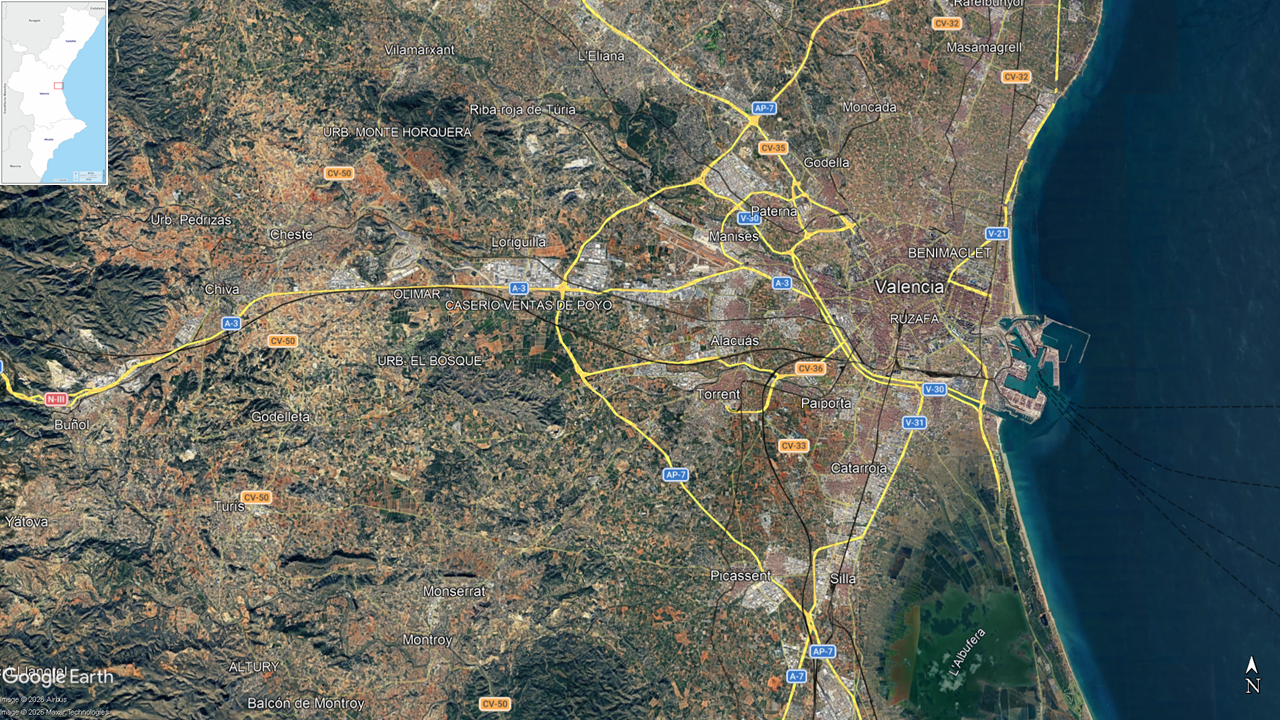
\includegraphics[width=0.9\textwidth]{images/results/topographic_overview.png}
    \caption{Topographic overview of the active $1311\text{ km}^2$ simulation domain overlaid on a Google Earth satellite composite.}
    \label{fig:topographic_overview}
\end{figure}

\subsection{Domain Discretization and Tensor Dimensions}

The entire simulation domain is discretized into a high-resolution uniform raster grid to preserve critical urban topographic 
micro-features—such as narrow streets, road underpasses, and structural barriers—that dictate the directional propagation of urban flood 
waves. The discretization and computational configuration are defined by the following specifications:

\begin{itemize}
    \item \textbf{Cell Spatial Resolution}: A cell size of $5\text{ m} \times 5\text{ m}$ is adopted uniformly across the domain. This 
    provides an optimal operational trade-off between local hydraulic precision and the high throughput required for real-time alerting 
    systems.

    \item \textbf{Tensor Structural Dimensions}: To ingest this topology into the deep learning and tensor math pipelines, the spatial 
    grid maps into a multi-channel tensor of approximately $5,500 \times 9,500$ cells per discrete property layer.

    \item \textbf{Temporal Step ($\Delta t$)}: To ensure numerical stability and strictly satisfy the Courant-Friedrichs-Lewy (CFL) 
    condition across highly dynamic, steep, and high-velocity open-channel flows, the execution engine enforces a fixed temporal step of 
    $\Delta t = 0.25$ seconds.
\end{itemize}

\subsection{Physical Fluid Properties and Flow Regime Selection}

To parameterize the fluid dynamics inside the cellular automata transition mechanics, the simulation enforces standard physical constants 
for water. These parameters are injected into the model architecture via global scalar configurations:

\begin{itemize}
    \item \textbf{Fluid Density ($\rho$)}: Set to a standard water density value of $1000.0\text{ kg/m}^3$.
    \item \textbf{Dynamic Fluid Viscosity ($\mu$)}: Set to $0.001\text{ Pa}\cdot\text{s}$ at standard ambient temperature.
\end{itemize}

Crucially, the interaction between these standard constants and the mathematical formulation of the transition rules enforces a 
deterministic regime selection. The underlying computational graph evaluates both a theoretical laminar viscous velocity ($v_{\text{lam}}$) 
and a turbulent open-channel velocity based on friction parameters ($v_{\text{turb}}$). The physical gating function inside the 
TensorFlow/ONNX engine approximates the effective cell velocity ($v_{\text{approx}}$) using a strict minimization selector:

\begin{equation}
    v_{\text{approx}} = \min\left(v_{\text{turb}}, v_{\text{lam}}\right)
\end{equation}

To demonstrate how these standard water scalars mathematically restrict the graph execution to the turbulent routing pathway under 
high-energy flash flood conditions, consider a representative inundated grid cell during the DANA event with a significant water depth 
($WD = 5.0\text{ m}$) and a steep surface slope gradient ($S_{\text{max}} = 5.0$). 

The theoretical laminar velocity component derived from viscous gravity-driven fluid layers is computed as:
\begin{equation}
    v_{\text{lam}} = \frac{\rho \cdot g \cdot WD^2 \cdot S_{\text{max}}}{3 \cdot \mu} = \frac{1000 \cdot 9.81 \cdot 5.0^2 \cdot 5.0}{3 \cdot 0.001} \approx 4 \times 10^8\text{ m/s}
\end{equation}

Conversely, the turbulent velocity component over a highly rough surface (e.g., a forested zone or heavily obstructed urban environment 
with a high Manning's roughness coefficient $n = 0.10$) is dictated by open-channel flow mechanics:

\begin{equation}
    v_{\text{turb}} = \frac{1}{n} \cdot WD^{2/3} \cdot \sqrt{S_{\text{max}}} = \frac{1}{0.10} \cdot 5.0^{2/3} \cdot \sqrt{5.0} \approx 65.38\text{ m/s}
\end{equation}

Applying the physical minimization gate to evaluate the effective cell propagation speed yields:

\begin{equation}
    v_{\text{approx}} = \min\left(65.38\text{ m/s},\; 4 \times 10^8\text{ m/s}\right) = 65.38\text{ m/s}
\end{equation}

As a consequence of injecting these standard fluid scalars, the laminar velocity component yields exceptionally high, non-physical values 
due to the low viscosity denominator ($\mu = 0.001$). This mathematically forces the TensorFlow/ONNX execution graph to bypass the laminar 
path and route all active, high-energy flood cell computations exclusively through the turbulent friction regime path, ensuring physical 
consistency across the entire flooded floodplain.
